\cleardoublepage
\mbox{}

\chapter{Implementación}
\label{ch:chapter4}

%\section{Paradigma de programación paralela OpenCL}

\section{Algoritmo ATDCA-GS en serie}

Anteriormente se ha presentado el problema que supone la existencia de firmas espectrales mixtas en varios píxeles de las imágenes hiperespectrales. La primera etapa del desmezclado espectral permite obtener los endmembers o firmas espectrales puras presentes, lo cual es necesario en la segunda etapa para el procesamiento posterior de la imagen y para la obtención de la presencia cuantitativa de dichos endmembers en cada pixel \cite{biblio:Spectral_unmixing_via}.

Como alternativa a la extracción de endmembers en la primera etapa, existen algoritmos orientados a la detección de targets, como es el caso del algoritmo ATDCA-GS implementado en este trabajo. Los targets son objetivos con características espectrales muy diferentes entre sí. Así, el conjunto de targets de una imagen ofrece una colección de firmas espectrales representativa de los distintos elementos que se pueden encontrar en la imagen.

Se puede realizar una similitud entre targets y endmembers puesto que estos últimos también representan una colección de firmas espectrales muy diferenciadas; sin embargo, es preciso destacar que los endmembers están asociados a firmas espectrales estrictamente puras mientras que los targets son una muestra representativa de los elementos presentes en la imagen.

Generalmente los algoritmos de detección de targets suelen funcionar de manera iterativa, obteniendo cada target en una iteración del algoritmo y, como resultado tras la ejecución, el conjunto de targets detectados. En algoritmos como el ATDCA también se requiere al comienzo una inicialización del conjunto de targets, siendo el píxel más brillante de la imagen (el de mayor intensidad) el más utilizado como primer target. Pese a no ser la única alternativa viable, se ha demostrado experimentalmente que dicho píxel siempre figura en el conjunto de píxeles de la solución \cite{biblio:y}, por lo que supone una elección correcta.

El algoritmo ATDCA usa el concepto de proyección ortogonal de un subespacio para hallar los targets en la imagen. Después de inicializarlo con el pixel más brillante, el siguiente objetivo será aquel con el valor de proyección más alto y será incluido en el subespacio para repetir el proceso tantas veces como targets se quieran detectar. Para optimizar el rendimiento del algoritmo, se ha empleado la ortogonalización de Gram Schmidt, que permite sustituir operaciones complejas, como invertir una matriz, por operaciones más simples y menos costosas en computación. En el Algoritmo~\ref{algoritmo atdca-gs vhdl} se muestra una implementación de este algoritmo en pseudocódigo.

\begin{algorithm}\small
\caption{Algoritmo ATDCA-GS}
\begin{algorithmic}[1]
\label{algoritmo atdca-gs vhdl}
%\STATE H $\leftarrow{}$ imagen hiperespectral de entrada
%\STATE nb $\leftarrow{}$ número de bandas de la imagen
%\STATE r $\leftarrow{}$ número de píxeles de la imagen
%\STATE w $\leftarrow{}$ un array de 1's en punto flotante de 32 bits
%\STATE t $\leftarrow{}$ número de targets a calcular
%\STATE P $\leftarrow{}$ array de posiciones de los targets en la imagen
%\STATE
\STATE \# Cálculo del píxel más brillante
\STATE max = 0
\FOR{$i=0 \text{ to } r-1$}
    \STATE brillo = H[:,i] * H[:,i]$^{T}$
    \IF{$brillo > max$}
        \STATE max = brillo
        \STATE pos = i
    \ENDIF
\ENDFOR
\STATE U[:,0] = H[:,pos]
\STATE P[0] = pos
\STATE
\STATE \# Cálculo del resto de targets
\FOR{$i=0 \text{ to } t-2$}
    \STATE UC = U[:,0..i]
    \IF{$i==0$}
        \STATE f[:,0] = $\sum_{k=0}^{nb-1}UC[k,0]$ / UC[nb,0]
        \STATE u[:,0] = UC[:,0]
        \STATE c2[0] = $\sum_{k=0}^{nb}u[k,0]$ / (u[:,0]$^{T}$ * u[:,0])
    \ELSE
        \STATE c1 = (u[:,0..(i-1)]$^{T}$ * UC[:,i]) / (u[:,0..(i-1)] * u[:,0..(i-1)])
        \STATE u[:, i] = UC[:,i] - $\sum_{k=0}^{i-1}(c1 * u[:,k])$
        \STATE c2 = $\sum_{k}(u[:,k])$ / (u[:,i]$^{T}$ * u[:,i])
        \STATE f[:,i] = w - $\sum_{k=0}^{i}(c2 * u[:,k])$
    \ENDIF
    \STATE
    \STATE max = 0
    \STATE \# Cálculo del píxel más diferente
    \FOR{$j=0 \text{ to } r-1$}
        \STATE result = f[:,i] * H[:,j]
        \STATE val = result$^{T}$ * result
        \IF{$val > max$}
            \STATE max = val
            \STATE pos = j
        \ENDIF
    \ENDFOR
    \STATE U[:,i+1] = H[:,pos]
    \STATE P[i+1] = pos
\ENDFOR
\end{algorithmic}
\end{algorithm}

\section{Paralelización y optimización del algoritmo ATDCA-GS usando VHDL}

Para la implementación en VHDL, se ha construido el módulo descrito gráficamente en la Figura~\ref{fig:modulo atdca-gs vhdl}. A continuación se muestra una secuencia de pasos del funcionamiento del algoritmo en VHDL y en las siguientes subsecciones se mostrarán los sub-componentes que se han empleado y una breve descripción de los mismos.

Usando como referencia el Algoritmo~\ref{algoritmo atdca-gs vhdl}, el código VHDL comienza utilizando los módulos Producto Escalar (línea 4) y Píxel Más Distinto (líneas 5 a 8) para calcular el píxel más brillante, esto es, el primer target de la solución.

Acto seguido se procede a calcular el segundo target empleando los módulos Producto Escalar Auxiliar en modo sólo suma y Divisor en la línea 17; y los módulos Producto Escalar Auxiliar en modo sólo suma, Producto Escalar y Divisor en la línea 19. Después de realizar estos cálculos, procede a calcular con ellos el píxel más distinto utilizando los módulos Producto Escalar Auxiliar en modo sólo multiplicación (línea 30) y Píxel Más Distinto (líneas 31 a 35).

Una vez obtenidos los dos primeros targets, el resto se calcularán haciendo uso de los módulos Producto Escalar, Producto Escalar Auxiliar en modo producto escalar y Divisor (línea 21); los módulos Array Resta Con Acumulación y Producto Escalar Auxiliar en modo sólo multiplicación (línea 22); los módulos Producto Escalar Aux en modo sólo suma, Registro Auxiliar, Producto Escalar y Divisor (línea 23); y los módulos Array Resta Con Acumulación y Producto Escalar Auxiliar en modo sólo multiplicación (línea 24). Después de realizar estos cálculos, se procede a calcular con ellos el píxel más distinto de la misma manera que ocurría para calcular el segundo target.

%[CARLOS - INICIO] Una vez que el algoritmo en serie esté descrito y antes de describir los módulos, pondría una especie de secuencia de pasos de cómo funciona el algoritmo en VHDL (así sirve para darle significado a los módulos aunque aun no se haya descrito su arquitectura)[CARLOS - FIN]

\begin{figure}
  \centering
    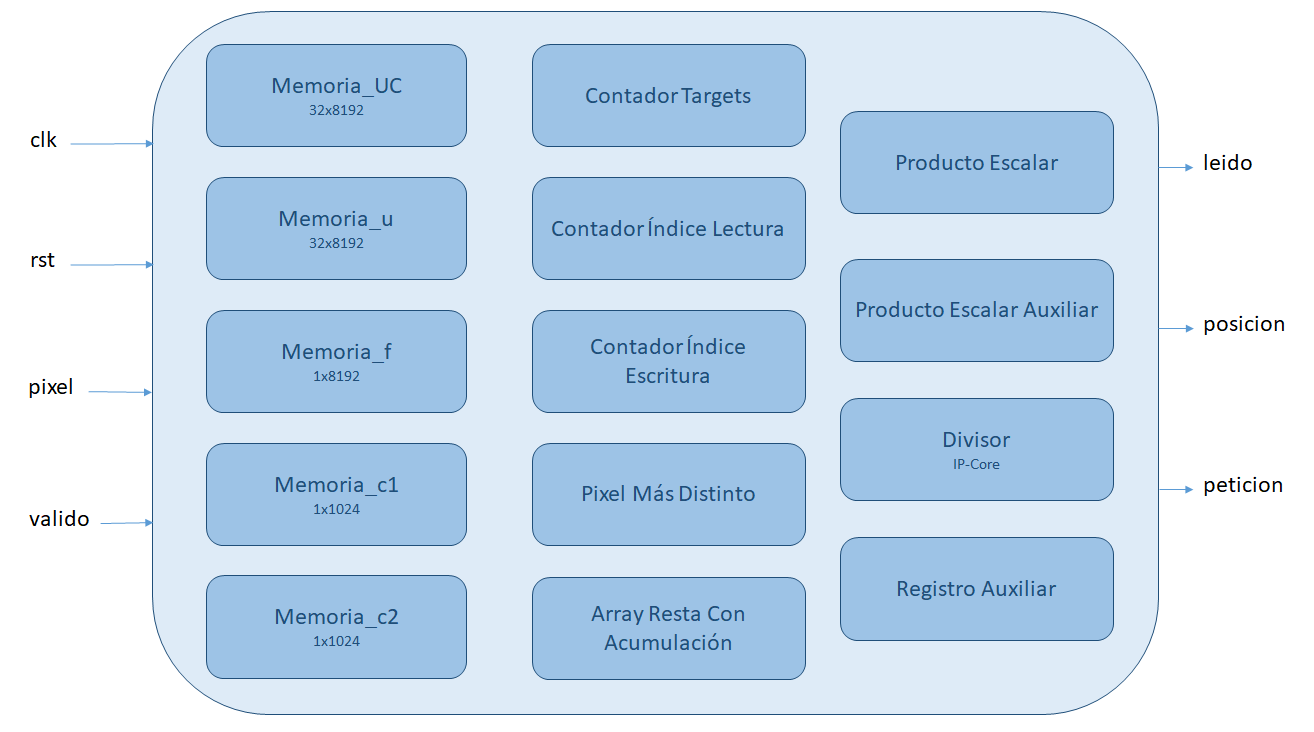
\includegraphics[width=1\textwidth]{Imagenes/DiagramaModuloATDCA-GS.png}
  \caption{Representación gráfica del módulo ATDCA-GS implementado en VHDL.}
  \label{fig:modulo atdca-gs vhdl}
\end{figure}

\subsection{IP-Cores}

Un IP-Core es un componente básico ya implementado que se encuentra incorporado en la herramienta IP-Core Generator dentro del software de desarrollo Xilinx ISE. La principal ventaja que presentan radica en que han sido específicamente diseñados para ser utilizados en dicha herramienta y, por consiguiente, ya han sido completamente optimizados. Se emplean durante el diseño de algoritmos para facilitar enormemente la construcción de operaciones matemáticas complejas y bloques de memoria.

A lo largo de la programación en VHDL del algoritmo ATDCA-GS se han utilizado algunos de los siguientes bloques IP-Core, cuya configuración y descripción se mostrará a continuación.

\subsubsection{Operadores de punto flotante}

Estos componentes hacen uso de una señal de entrada llamada operation$\_$nd, que indica al módulo que los operadores ya están disponibles y debe comenzar a realizar los cálculos. También hacen uso de una señal de salida llamada rdy (ready), que indica que el componente ha terminado de operar y el resultado está ya disponible.

Estos módulos se han utilizado para trabajar con números en punto flotante de precisión simple (32 bits) y están segmentadas, es decir, admiten la entrada de una secuencia consecutiva de datos. Tras una latencia inicial, se irá produciendo un resultado en cada ciclo y en el mismo orden que llevaba la secuencia de entrada.

\begin{itemize}
    \item Restador (restadorPF32Bits.xco)
        \begin{itemize}
            \item IP-core: Floating-point.
            \item Functions: Add/Substract (Substract).
            \item Floating-point precision of A/B inputs: single (32 bits).
            \item Architecture optimizations: Low latency.
            \item Family optimizations: No usage (= Logic only).
            \item Latency: 0.
            \item Cycles per operation: 1.
        \end{itemize}
    \item Divisor (div$\_$escalar$\_$PF32Bits.xco)
        \begin{itemize}
            \item IP-core: Floating-point.
            \item Functions: Divide.
            \item Floating-point precision of A/B inputs: single (32 bits).
            \item Architecture optimizations: High speed.
            \item Family optimizations: No usage (= Logic only).
            \item Latency: Use maximum latency (28).
            \item Cycles per operation: 1.
        \end{itemize}
    \item Comparador (cmp$\_$mayor.xco)
        \begin{itemize}
            \item IP-core: Floating-point.
            \item Functions: Compare (Greater than).
            \item Floating-point precision of A/B inputs: single (32 bits).
            \item Architecture optimizations: High speed.
            \item Family optimizations: No usage (= Logic only).
            \item Latency: 0.
            \item Cycles per operation: 1.
        \end{itemize}
    \item Sumador (sumadorPF32Bits.xco)
        \begin{itemize}
            \item IP-core: Floating-point.
            \item Functions: Add/Substract (Add).
            \item Floating-point precision of A/B inputs: single (32 bits).
            \item Architecture optimizations: High speed.
            \item Family optimizations: Full usage (= 2 x DSP48E).
            \item Latency: 2.
            \item Cycles per operation: 1.
        \end{itemize}
    \item Multiplicador (multiplicadorPF32Bits.xco)
        \begin{itemize}
            \item IP-core: Floating-point.
            \item Functions: Multiply.
            \item Floating-point precision of A/B inputs: single (32 bits).
            \item Architecture optimizations: High speed.
            \item Family optimizations: Full usage (= 2 x DSP48E).
            \item Latency: 1.
            \item Cycles per operation: 1.
        \end{itemize}
\end{itemize}

\subsubsection{Bloques de memoria}

Estos componentes son bloques de memoria que permiten seleccionar un tamaño y unas características concretas tales como los tipos de puertos o la prioridad de lectura o escritura. De esta manera se han podido diseñar bloques de memoria específicos según las necesidades del algoritmo. En concreto, se han utilizado 4 bloques de memoria distintos:

\begin{itemize}
    \item Memoria 2x4096 2 True Dual Port (memoria2x4096$\_$WRITE$\_$FIRST.xco)
        \begin{itemize}
            \item IP-core: Block Memory Generator.
            \item Memory type: True Dual Port RAM.
            \item Port A - Read/Write width: 4096.
            \item Port A - Read/Write depth: 2.
            \item Port A - Operating mode: Write first.
            \item Port B - Read/Write width: 4096.
            \item Port B - Read/Write depth: 2.
            \item Port B - Operating mode: Write first.
        \end{itemize}
    \item Memoria 1x1024 (mem1x1024.xco)
        \begin{itemize}
            \item IP-core: Block Memory Generator.
            \item Memory type: Simple Dual Port RAM.
            \item Common clock.
            \item Port A - Write width: 1024.
            \item Port A - Write depth: 2.
            \item Port A - Operating mode: Read first.
            \item Port B - Read width: 1024.
            \item Port B - Read depth: 2.
            \item Port B - Operating mode: Read first.
            \item Fill Remaining Memory Locations: 0 (Hex).
        \end{itemize}
    \item Memoria 2x4096 Simple Dual Port (memoria2x4096.xco)
        \begin{itemize}
            \item IP-core: Block Memory Generator.
            \item Memory type: Simple Dual Port RAM.
            \item Port A - Write width: 4096.
            \item Port A - Write depth: 2.
            \item Port A - Operating mode: Write first.
            \item Port B - Read width: 4096.
            \item Port B - Read depth: 2.
            \item Port B - Operating mode: Write first.
        \end{itemize}
    \item Memoria 32x4096 (memoria.xco)
        \begin{itemize}
            \item IP-core: Block Memory Generator.
            \item Memory type: Simple Dual Port RAM.
            \item Port A - Write width: 4096.
            \item Port A - Write depth: 32.
            \item Port A - Operating mode: Write first.
            \item Port B - Read width: 4096.
            \item Port B - Read depth: 32.
            \item Port B - Operating mode: Write first.
            \item Fill Remaining Memory Locations: 0 (Hex).
        \end{itemize}
\end{itemize}

\subsection{Módulos VHDL}

A continuación se definen los módulos VHDL que se han implementado para este trabajo.

\subsubsection{Memoria 32x8192 (mem$\_$32x8192.vhd)}

\begin{itemize}
    \item DESCRIPCIÓN
        \begin{itemize}
            \item Memoria de doble puerto simple, es decir, permite realizar una escritura (puerto A) y una lectura (puerto B) simultáneamente. Combina dos memorias de 32x4096 para generar una de 32x8192. Tiene una política de Write First, lo que significa que la lectura garantiza que el dato leído esté siempre actualizado. Está estructurada para almacenar datos de 8192 bits, que sirven para representar un máximo de 256 bandas de 32 bits cada una. Esos 32 bits son los necesarios para representar un número en punto flotante de precisión simple. Tiene 32 filas, una por cada target que se vaya a detectar y almacenar durante la ejecución del algoritmo. No se esperan más de 32 como máximo.
        \end{itemize}
    \item INPUT
        \begin{itemize}
            \item clka: señal de reloj del puerto A.
            \item wea: señal Write Enable que indica si se debe realizar una escritura (1) o no (0).
            \item addra: señal de 5 bits que indica la dirección de memoria sobre la que va a trabajar el puerto A.
            \item dina: señal de 8192 bits que indica el dato que entra por el puerto A.
            \item clkb: señal de reloj del puerto B.
            \item addrb: señal de 5 bits que indica la dirección de memoria sobre la que va a trabajar el puerto B.
        \end{itemize}
    \item OUTPUT
        \begin{itemize}
            \item doutb: señal de 8192 bits que indica el dato que sale por el puerto B.
        \end{itemize}
    \item UTILIZADO EN
        \begin{itemize}
            \item Memoria UC.
            \item Memoria u.
        \end{itemize}
\end{itemize}

\subsubsection{Memoria 1x8192 (mem$\_$1x8192.vhd)}

\begin{itemize}
    \item DESCRIPCIÓN
        \begin{itemize}
            \item Memoria de doble puerto simple, es decir, permite realizar una escritura (puerto A) y una lectura (puerto B) simultáneamente. Combina dos memorias de 2x4096 para generar una de 1x8192. Tiene una política de Write First, lo que significa que la lectura garantiza que el dato leído esté siempre actualizado. Está estructurada para almacenar datos de 8192 bits, que sirven para representar un máximo de 256 bandas de 32 bits cada una. Esos 32 bits son los necesarios para representar un número en punto flotante de precisión simple. Tiene 2 filas pero sólo se utilizará una. Esta fila almacenará la proyección calculada en cada iteración del algoritmo.
        \end{itemize}
    \item INPUT
        \begin{itemize}
            \item clka: señal de reloj del puerto A.
            \item wea: señal Write Enable que indica si se debe realizar una escritura (1) o no (0).
            \item addra: señal de 1 bit que indica la dirección de memoria sobre la que va a trabajar el puerto A.
            \item dina: señal de 8192 bits que indica el dato que entra por el puerto A.
            \item clkb: señal de reloj del puerto B.
            \item addrb: señal de 1 bit que indica la dirección de memoria sobre la que va a trabajar el puerto B.
        \end{itemize}
    \item OUTPUT
        \begin{itemize}
            \item doutb: señal de 8192 bits que indica el dato que sale por el puerto B.
        \end{itemize}
    \item UTILIZADO EN
        \begin{itemize}
            \item Memoria f.
        \end{itemize}
\end{itemize}

\subsubsection{Memoria c (memoriac.vhd)}

\begin{itemize}
    \item DESCRIPCIÓN
        \begin{itemize}
            \item Memoria de doble puerto simple, es decir, permite realizar una escritura (puerto A) y una lectura (puerto B) simultáneamente. Tiene una política de Read First, lo que significa que la lectura garantiza que el dato leído no sea el sobreescrito por la escritura. Está estructurada para almacenar datos de 32 bits agrupados dentro de una única fila de 1024 bits. Por tanto, se representan 32 números (número máximo de targets) de 32 bits cada uno. Esos 32 bits son los necesarios para representar un número en punto flotante de precisión simple. Tiene 2 filas pero sólo se utilizará una. Esta fila almacenará el cálculo generado para el target que corresponda en cada momento en función de la iteración del algoritmo en la que nos encontremos.
        \end{itemize}
    \item INPUT
        \begin{itemize}
            \item clk: señal de reloj del puerto A.
            \item wea: señal Write Enable que indica si se debe realizar una escritura (1) o no (0).
            \item pos: señal de 5 bits que indica qué 32 bits de la única fila de la memoria deben ser modificados en la escritura.
            \item dina: señal de 32 bits que indica el dato que entra por el puerto A.
        \end{itemize}
    \item OUTPUT
        \begin{itemize}
            \item doutb: señal de 1024 bits que indica el dato que sale por el puerto B.
        \end{itemize}
    \item UTILIZADO EN
        \begin{itemize}
            \item Memoria c1.
            \item Memoria c2.
        \end{itemize}
\end{itemize}

\subsubsection{Contador (contador$\_$rst.vhd)}

\begin{itemize}
    \item DESCRIPCIÓN
        \begin{itemize}
            \item Contador módulo n comenzando desde 0. En cada flanco de reloj, si la señal count$\_$up está a 1, se suma 1 al valor actual del contador. Si está a 0, no se produce ningún cambio. Por la señal dout sale el valor por el que vaya la cuenta del contador en cada flanco de reloj. Las señales rst y rst$\_$sync, si están a 1, reinician el contador haciendo que la cuenta comience de nuevo en 0.
        \end{itemize}
    \item GENÉRICOS
        \begin{itemize}
            \item n = 32: número de bits del contador.
        \end{itemize}
    \item INPUT
        \begin{itemize}
            \item clk: señal de reloj.
            \item rst: señal de reset asíncrona.
            \item rst$\_$sync: señal de reset síncrona.
            \item count$\_$up: señal que indica si se aumenta el valor del contador o se deja tal y como está.
        \end{itemize}
    \item OUTPUT
        \begin{itemize}
            \item dout: señal de n-1 bits indicando la cuenta por la que va el contador.
        \end{itemize}
    \item UTILIZADO EN
        \begin{itemize}
            \item Contador de Targets.
            \item Contador de Índice de Lectura.
            \item Contador de Índice de Escritura.
            \item Contador en el módulo Pixel Más Distinto.
        \end{itemize}
\end{itemize}

\subsubsection{Producto Escalar (mult$\_$sum$\_$PF32Bits.vhd)}

\begin{figure}
  \centering
    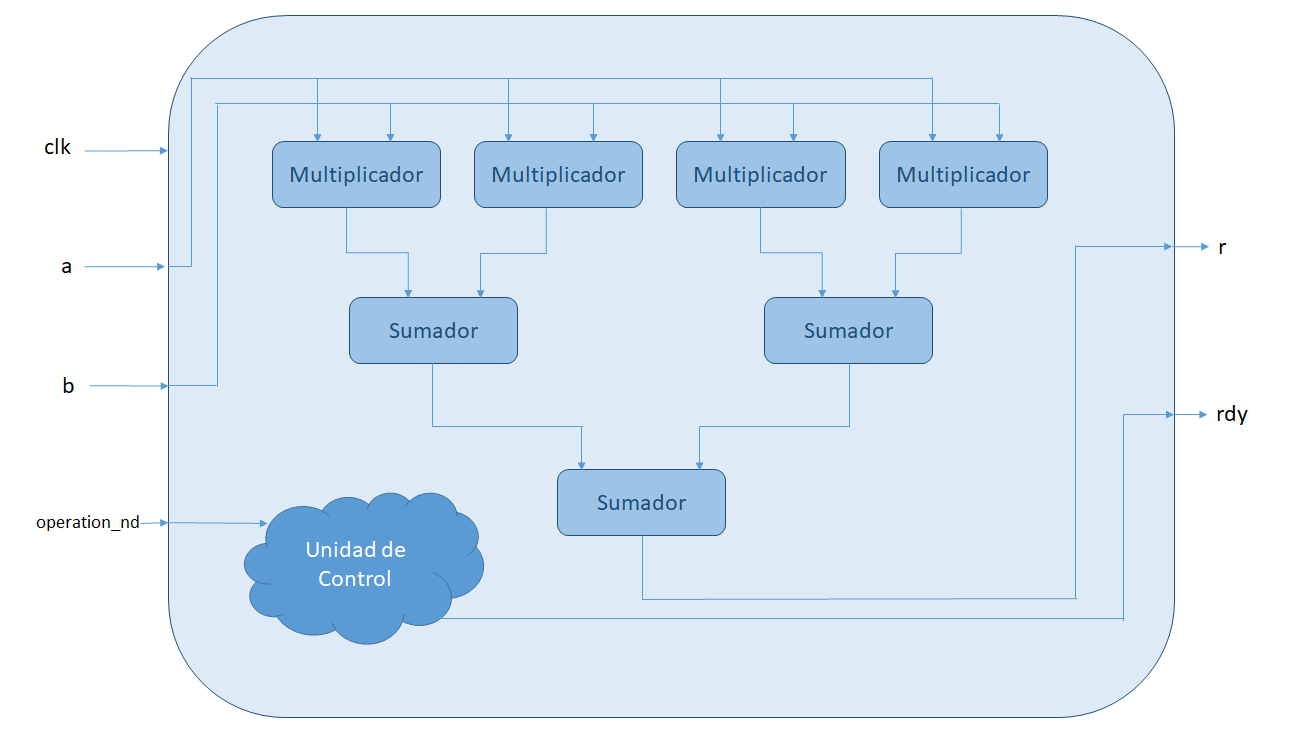
\includegraphics[width=1\textwidth]{Imagenes/DiagramaModuloProductoEscalar.png}
  \caption{Representación gráfica de un ejemplo del módulo Producto Escalar implementado en VHDL.}
  \label{fig:modulo producto escalar vhdl}
\end{figure}

\begin{itemize}
    \item DESCRIPCIÓN
        \begin{itemize}
            \item Realiza el producto escalar de las dos entradas A y B, que serán dos vectores de Nx32 bits. Se utilizan N multiplicadores, uno por cada multiplicación A[i]xB[i], y, posteriormente, un árbol de sumadores conectado a los resultados de los multiplicadores, obteniendo al final un numero de 32 bits que indica el producto escalar de los vectores A y B. Cuando el resultado está disponible, se muestra por la salida r en el siguiente flanco de reloj. Se puede observar gráficamente un ejemplo de este módulo para N = 4 en la Figura~\ref{fig:modulo producto escalar vhdl}.
        \end{itemize}
    \item GENÉRICOS
        \begin{itemize}
            \item N = 4: número de elementos que tiene cada vector. Para el algoritmo no se utilizará este valor, sino el número de bandas.
            \item N$\_$log2 = 2: logaritmo en base 2 de N. Para el algoritmo no se utilizará este valor sino el logaritmo en base 2 del número de bandas.
        \end{itemize}
    \item INPUT
        \begin{itemize}
            \item clk: señal de reloj.
            \item a: señal de Nx32 bits indicando el vector A.
            \item b: señal de Nx32 bits indicando el vector B.
            \item operation$\_$nd: señal que indica si los operandos están disponibles.
        \end{itemize}
    \item OUTPUT
        \begin{itemize}
            \item r: señal de 32 bits indicando el resultado del producto escalar de los vectores A y B.
            \item rdy: señal que indica que el resultado ya se encuentra disponible.
        \end{itemize}
    \item UTILIZADO EN
        \begin{itemize}
            \item ATDCA-GS.
        \end{itemize}
\end{itemize}

\subsubsection{Producto Escalar Auxiliar (mult$\_$sum$\_$aux$\_$PF32Bits.vhd)}

\begin{figure}
  \centering
    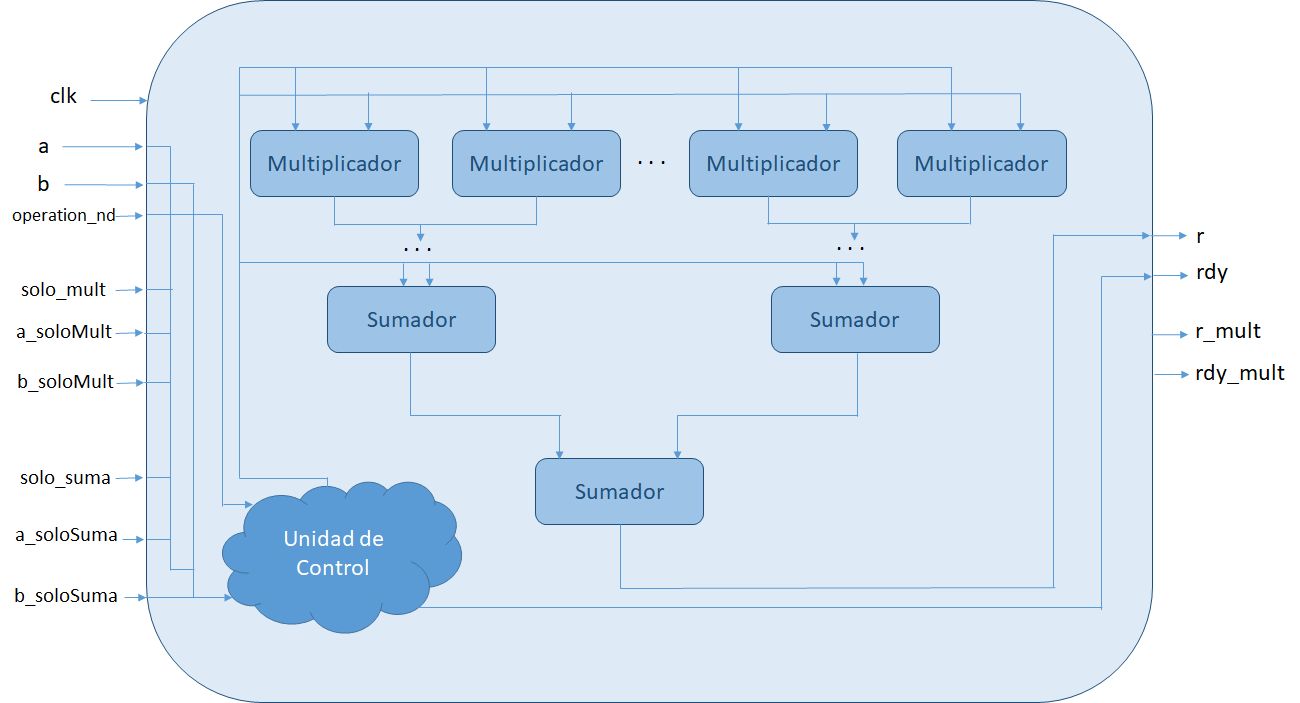
\includegraphics[width=1\textwidth]{Imagenes/DiagramaModuloProductoEscalarAuxiliar.png}
  \caption{Representación gráfica de un ejemplo del módulo Producto Escalar Auxiliar implementado en VHDL.}
  \label{fig:modulo producto escalar auxiliar vhdl}
\end{figure}

\begin{itemize}
    \item DESCRIPCIÓN
        \begin{itemize}
            \item En caso de que solo$\_$suma y solo$\_$mult estén a 0, realiza exactamente la misma funcionalidad que el módulo Producto Escalar. En caso de que solo$\_$suma esté a 1, realiza la suma de todos los elementos de los dos vectores de entrada, A y B, empleando para ello un árbol de sumadores. Cuando el resultado está disponible, se muestra por la salida r en el siguiente flanco de reloj y la señal rdy se pone a 1. En caso de que solo$\_$mult esté a 1, realiza la multiplicación elemento a elemento de los dos vectores de entrada. Cuando se obtiene el resultado, se muestra por la señal r$\_$mult (de Nx32 bits) y la señal rdy$\_$mult se pone a 1. Se puede observar gráficamente un ejemplo de este módulo en la Figura~\ref{fig:modulo producto escalar auxiliar vhdl}.
        \end{itemize}
    \item GENÉRICOS
        \begin{itemize}
            \item N = 256: número de elementos que tiene cada vector (equivaldrá al número de bandas de la imagen).
            \item N$\_$log2 = 8: logaritmo en base 2 de N.
        \end{itemize}
    \item INPUT
        \begin{itemize}
            \item clk: señal de reloj.
            \item a: señal de Nx32 bits indicando el vector A.
            \item b: señal de Nx32 bits indicando el vector B.
            \item operation$\_$nd: señal que indica si los operandos están disponibles.
            \item solo$\_$mult: indica si se debe realizar la multiplicación elemento a elemento o no.
            \item solo$\_$suma: indica si se debe realizar la suma en árbol o no.
            \item a$\_$soloSuma: señal de Nx32 bits indicando el vector A para la operación de suma en árbol.
            \item b$\_$soloSuma: señal de Nx32 bits indicando el vector B para la operación de suma en árbol.
            \item a$\_$soloMult: señal de Nx32 bits indicando el vector A para la operación de multiplicación elemento a elemento.
            \item b$\_$soloMult: señal de Nx32 bits indicando el vector B para la operación de multiplicación elemento a elemento.
        \end{itemize}
    \item OUTPUT
        \begin{itemize}
            \item r: señal de 32 bits indicando el resultado de la operación suma en árbol o la de producto escalar (la que se haya realizado) de los vectores A y B.
            \item rdy: señal que indica que el resultado de la operación suma en árbol o la de producto escalar (la que se haya realizado) ya se encuentra disponible.
            \item r: señal de 32 bits indicando el resultado de la operación de multiplicación elemento a elemento de los vectores A y B.
            \item rdy$\_$mult: señal que indica que el resultado de la operación de multiplicación elemento a elemento ya se encuentra disponible.
        \end{itemize}
    \item UTILIZADO EN
        \begin{itemize}
            \item ATDCA-GS.
        \end{itemize}
\end{itemize}

\subsubsection{Registro (registro$\_$rst.vhd)}

\begin{itemize}
    \item DESCRIPCIÓN
        \begin{itemize}
            \item En cada flanco de reloj, si la señal load está a 1, se introduce el dato de la señal din en el registro. Si está a 0, no se produce esta actualización. Por la señal dout sale lo que haya dentro del registro en cada flanco de reloj con una política de Read First, lo que significa que, si se ha actualizado el contenido del registro (load = 1), será el nuevo dato el que saldrá por dout en ese mismo instante de tiempo. Las señales rst y rst$\_$sync, si están a 1, reinician el registro haciendo que el contenido del mismo sean 0’s.
        \end{itemize}
    \item GENÉRICOS
        \begin{itemize}
            \item n = 32: número de bits de los datos que se almacenan en el registro.
        \end{itemize}
    \item INPUT
        \begin{itemize}
            \item clk: señal de reloj.
            \item rst: señal de reset asíncrona.
            \item rst$\_$sync: señal de reset síncrona.
            \item load: señal que indica si se actualiza el valor del registro o se deja tal y como está.
            \item din: señal de n bits indicando el dato a introducir en el registro.
        \end{itemize}
    \item OUTPUT
        \begin{itemize}
            \item dout: señal de n bits indicando el dato que se encuentra almacenado en el registro.
        \end{itemize}
    \item UTILIZADO EN
        \begin{itemize}
            \item Registro Mayor Valor en el módulo Pixel Más Distinto.
            \item Registro Mayor Posición en el módulo Pixel Mas Distinto.
            \item Registro Auxiliar.
        \end{itemize}
\end{itemize}

\subsubsection{Pixel Más Distinto (pixel$\_$mas$\_$distinto.vhd)}

\begin{figure}
  \centering
    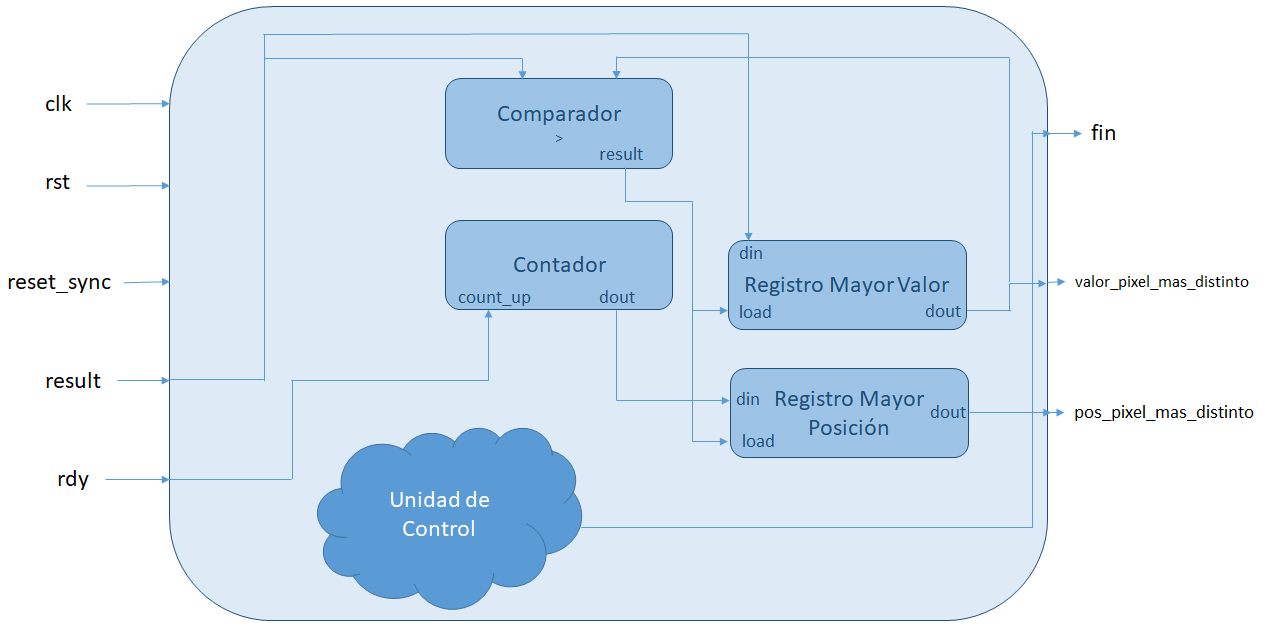
\includegraphics[width=1\textwidth]{Imagenes/DiagramaModuloPixelMasDistinto.png}
  \caption{Representación gráfica del módulo Pixel Más Distinto implementado en VHDL.}
  \label{fig:modulo pixel mas distinto vhdl}
\end{figure}

\begin{itemize}
    \item DESCRIPCIÓN
        \begin{itemize}
            \item Recibe un número de píxeles y calcula cuál de ellos es el más brillante (o distinto), es decir, el que tiene mayor valor. Para ello hace uso de dos registros, un contador y un comparador que indica si el operando A es mayor que el operando B. Se puede observar gráficamente la estructura de este módulo en la Figura~\ref{fig:modulo pixel mas distinto vhdl}.
        \end{itemize}
    \item GENÉRICOS
        \begin{itemize}
            \item NUMPIXELES = 2: número de pixeles que se van a analizar. El algoritmo sobreescribirá este valor según el número de pixeles sobre el que se ejecute.
            \item NUM$\_$PIXELES$\_$log2 = 1: logaritmo en base dos del número de píxeles. El algoritmo sobreescribirá este valor según el número de pixeles sobre el que se ejecute.
        \end{itemize}
    \item INPUT
        \begin{itemize}
            \item clk: señal de reloj.
            \item rst: señal de reset asíncrona.
            \item reset$\_$sync: señal de reset síncrona.
            \item result: señal de 32 bits indicando el siguiente pixel a analizar.
            \item rdy: señal que indica que el siguiente pixel a analizar ya se encuentra disponible.
        \end{itemize}
    \item OUTPUT
        \begin{itemize}
            \item fin: señal que indica que ya se han analizado todos los píxeles y ya se ha encontrado el pixel más distinto.
            \item pos$\_$pixel$\_$mas$\_$distinto: señal de NUM$\_$PIXELES$\_$log2 bits que indica la posición en la memoria del pixel más distinto que se ha encontrado.
            \item valor$\_$pixel$\_$mas$\_$distinto: señal de 32 bits que indica el valor del pixel más distinto que se ha encontrado.
        \end{itemize}
    \item UTILIZADO EN
        \begin{itemize}
            \item ATDCA-GS.
        \end{itemize}
\end{itemize}

\subsubsection{Array Resta con Acumulación (array$\_$restadores$\_$con$\_$acumulacion$\_$PF32Bits.vhd)}

\begin{figure}
  \centering
    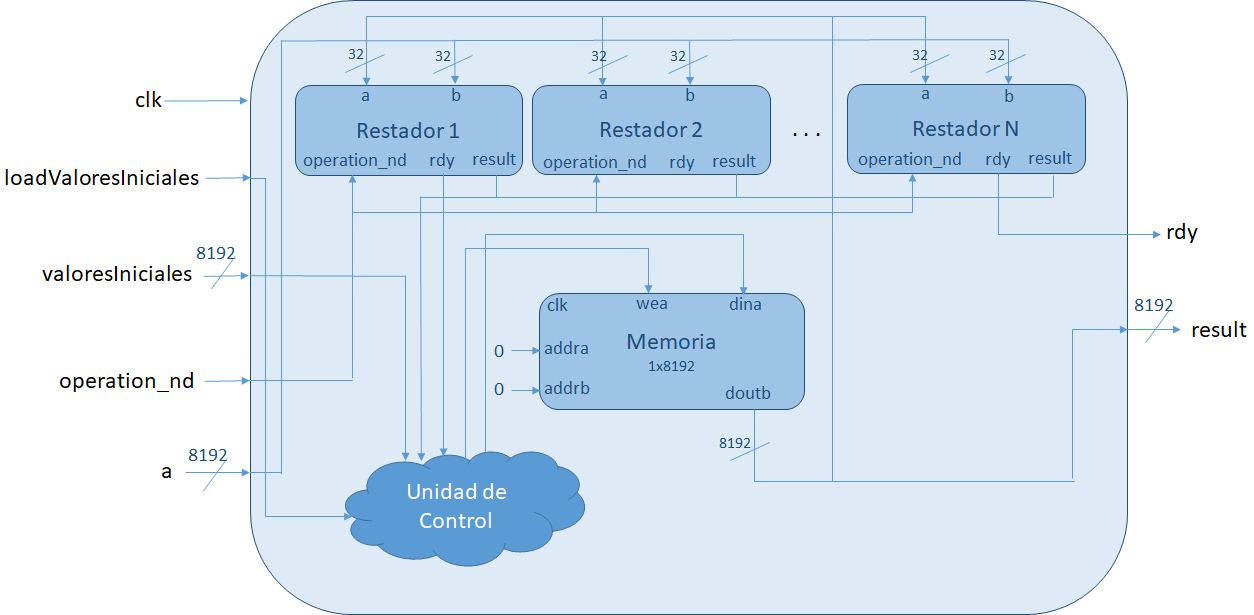
\includegraphics[width=1\textwidth]{Imagenes/DiagramaModuloArrayRestaConAcumulacion.png}
  \caption{Representación gráfica del módulo Array Resta Con Acumulación implementado en VHDL.}
  \label{fig:modulo array resta con acumulacion vhdl}
\end{figure}

\begin{itemize}
    \item DESCRIPCIÓN
        \begin{itemize}
            \item Recibe un operando de Nx32 bits y lo resta a un valor que puede ser, o bien un valor inicial cargado previamente a los cálculos, o bien el resultado acumulado de las operaciones anteriores. La resta se realiza como si fuera una operación elemento a elemento de dos vectores de N números en punto flotante, por lo que se utilizan N restadores. Para almacenar el valor acumulado se hace uso de una memoria de 1x8192 bits. Se puede observar gráficamente la estructura de este módulo en la Figura~\ref{fig:modulo array resta con acumulacion vhdl}.
        \end{itemize}
    \item GENÉRICOS
        \begin{itemize}
            \item N = 256: número de restadores que se van a utilizar (el equivalente al número de bandas de la imagen hiperespectral).
        \end{itemize}
    \item INPUT
        \begin{itemize}
            \item clk: señal de reloj.
            \item loadValoresInciales: señal que indica si se cargan los valores iniciales o no.
            \item valoresInciales: señal de Nx32 bits que representa los valores iniciales que deben cargarse cuando sea necesario.
            \item operation$\_$nd: señal que indica si los operandos están disponibles para las restas.
            \item a: señal de Nx32 bits que representa los N elementos que se desean restar a los valores acumulados hasta el momento.
        \end{itemize}
    \item OUTPUT
        \begin{itemize}
            \item result: señal de Nx32 bits indicando el resultado de las operaciones.
            \item rdy: señal que indica que el resultado de las operaciones ya se encuentra disponible.
        \end{itemize}
    \item UTILIZADO EN
        \begin{itemize}
            \item ATDCA-GS.
        \end{itemize}
\end{itemize}

\section{Paralelización y optimización del algoritmo ATDCA-GS usando OpenCL}

Se ha realizado el estudio de una implementación paralela del algoritmo usando el paradigma OpenCL para su posterior optimización\footnote{https://www.intel.com/content/dam/www/programmable/us/en/pdfs/literature/hb/opencl-sdk/aocl-best-practices-guide.pdf}. Antes de continuar con el estudio, se comentará una serie de conceptos relacionados con el paradigma de progrmación OpenCL.

La especificación de OpenCL\footnote{https://www.khronos.org/opencl} fue desarrollada para permitir una libertad en términos de implementar aplicaciones que podrían ejecutarse en diferentes arquitecturas. En el paradigma OpenCL, el programa ``host'', está a cargo de las operaciones de E/S, inicialización de datos y controlando el ``device''. Además, lanza los códigos ``kernel'' y la sincronización entre ellos. Entre los principales beneficios se encuentra el amplio rango de dispositivos hardware a ser usados: CPUs, GPUs y FPGAs. Todos ellos podrán ser usados con un esfuerzo moderado en el proceso de codificación.

\begin{figure}[htb]
\centering
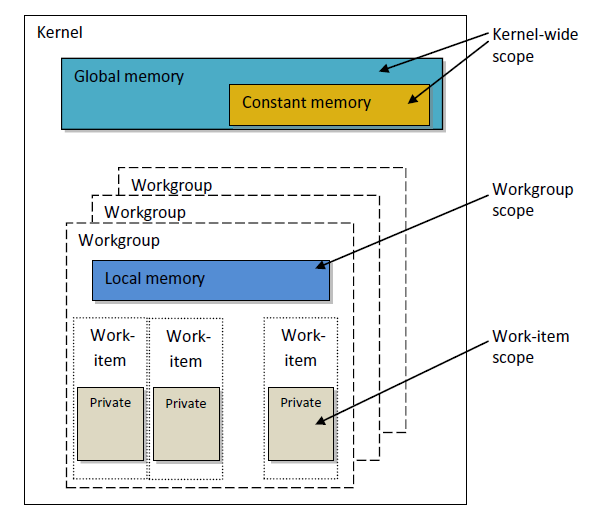
\includegraphics[width=0.75\textwidth]{images/imagen_jerarquia.PNG}
\caption{Jerarquía de memoria en OpenCL, y división en \textit{work-items}.} \label{fig:imagen_jerarquia}
\end{figure}

Un kernel OpenCL permite expresar paralelismo a través de la ejecución de varios \textit{work-items}. Un grupo de \textit{work-items} forman un textit{work-group} que corre sobre una unidad de cómputo individual o ``single compute unit''. Los \textit{work-items} ejecutan el mismo \textit{kernel}  (con un único id), comparte una memoria rápida denominada \textit{local memory} (ver Figura \ref{fig:imagen_jerarquia}\footnote{https://www.mql5.com/es/articles/407}) y puede ser sincronizada con barreras. La dimensión máxima de cada {work-group} dependerá de la especificación del \textit{device} usado (ver Sección \ref{ch:chapte5}).   

Una vez que se han conocido los conceptos relacionados con el paradigma de programación paralela OpenCL, pasaremos a analizar una implementación previa en OpenCL del algoritmo ATDCA-GS. En este trabajo previo \cite{portabilitySPIE_Sergio} fueron implementados tres kernels: cálculo del píxel más brillante, cálculo de la proyección ortogonal de cada píxel sobre la imagen y obtención de la máxima proyección ortogonal. De cada uno de ellos se mostrará a continuación el pseudocódigo que se ha seguido.

%Para su implementación en OpenCL se ha realizado un perfilado del código optimizado en lenguaje C. A través de este estudio se ha podido encontrar las distintas porciones de código candidatas a paralelizar, ya que podrían llegar a ser posibles cuellos de botella de rendimiento o también conocido como "bottlenecks". Se han encontrado hasta un total de 3 zonas de códigos donde una correcta paralelización puede suponer una mejora en el rendimiento. Estas zonas son: cálculo del píxel más brillante, cálculo de la proyección ortogonal de un píxel sobre la imagen y obtención de la máxima proyección ortogonal. Para cada una de las zonas identificadas, un \textit{kernel} será implementado.

El primer \textit{kernel} sobre el que se ha realizado el estudio, es el correspondiente al cálculo del píxel más brillante. El pseudocódigo estudiado es el descrito en el algoritmo \ref{kernel_brightest_opencl}. Tras analizarlo y teniendo en cuenta que esta parte consume aproximadamente el \textbf{5\%} del tiempo de procesamiento total del algoritmo considerando una imagen hiperespectral real como es Cuprite, se han tenido en cuenta varias consideraciones: 

\begin{algorithm}[htb]\small
\caption{Cálculo del píxel más brillante}
\begin{algorithmic}[1]
\label{kernel_brightest_opencl}
\STATE global d$\_$image $\leftarrow{}$ Vector inicial $\textbf{X}$$[r]$, d$\_$bright $\leftarrow{}$ El valor brillo de cada píxel\\
\STATE registers bright $\leftarrow{}$ 0, value $\leftarrow{}$ 0\\
\STATE id $\leftarrow{}$ get\_group\_id(0) * get\_local\_size(0) +
get\_local\_id(0)\\
\% $n_{b}$ indica el número de bandas espectrales\\ 
\IF{$id < r$} 
\FOR{$k=0 \text{ to } n_{b}$}
\STATE value $\leftarrow{}$ d$\_$image[id + (k * r)]\\
\STATE bright $\leftarrow{}$ bright + value * value\\
\ENDFOR 
\STATE d$\_$bright[id] $\leftarrow{}$ bright\\
\ENDIF
\end{algorithmic}
\end{algorithm}

\begin{enumerate}
\item Empleo de \textit{restrict} en arrays usados en memoria global. De esta manera se evita que los punteros no estén apuntando a ubicaciones en memoria con información. A la hora de definir los parámetros de la función kernel se ha acompañado la variable \textit{restrict} a los arrays declarado en memoria global (\textit{restrict d\_image} y \textit{restrict d\_bright}).
%\item Uso de relleno adicional o \textit{padding} en arrays.
\item Distribución óptima de los datos para favorecer la vectorización. Para ello, la línea 6 del Algoritmo \ref{kernel_brightest_opencl} se ha modificado por lo siguiente: d$\_$image[k + (id * $n_{b}$)].
\item Desenrollado de bucles (\textit{loop unrolling}). Entre las líneas 4 y 5 del Algoritmo \ref{kernel_brightest_opencl} se ha introducido la siguiente directiva: \#\textit{pragma unroll num\_factor}, permitiendo un factor diferente para el desenrollado del bucle dependiendo del tamaño de la imagen. 
\end{enumerate}

\begin{algorithm}[htb]\small
\caption{Reducción para obtener la máxima proyección ortogonal}
\begin{algorithmic}[1]
\label{kernel_reduction}
\STATE global d$\_$bright, d$\_$projection, d$\_$index\\
\STATE local s$\_$p[BLK] $\leftarrow{}$Estructura inicial para almacenar todas las proyecciones\\
\STATE local s$\_$i[BLK] $\leftarrow{}$Estructura inicial para almacenar todos los índices para cada proyección\\
\STATE tid $\leftarrow{}$ get\_local\_id(0)\\
\STATE id $\leftarrow{}$ get\_group\_id(0)  * (get\_local\_size(0) * 2) + get\_local\_id(0)\\
\IF{(id + get\_local\_size(0)) $\ge$ r}
	\STATE s$\_$p[tid] $\leftarrow{}$ d$\_$bright[id]
	\STATE s$\_$i[tid] $\leftarrow{}$ id
\ELSE
	\IF{d$\_$bright[id] $>$ d$\_$bright[id + get\_local\_size(0)]}
		\STATE s$\_$p[tid] $\leftarrow{}$ d$\_$bright[id]
		\STATE s$\_$i[tid] $\leftarrow{}$ id
    \ELSE
    	\STATE s$\_$p[tid] $\leftarrow{}$ d$\_$bright[id + get\_local\_size(0)]
		\STATE s$\_$i[tid] $\leftarrow{}$ (id + get\_local\_size(0))
	\ENDIF
\ENDIF

\STATE barrier($\text{CLK\_LOCAL\_MEM\_FENCE}$)\\

\% En esta sincronización, todos los hilos deben esperar la ejecución de todos los hilos en un bloque para poder completar la copia en memoria local de s$\_$p y s$\_$i

\FOR{s=get\_local\_size(0) / 2 $\text{ to }$ {s$>$0; s$>>$=1}}
	\IF{tid $<$ s}
    	\IF{s$\_$p[tid] $\le$ s$\_$p[tid + s]}
    		\STATE s$\_$p[tid] $\leftarrow{}$ s$\_$p[tid + s]
			\STATE s$\_$i[tid] $\leftarrow{}$ s$\_$i[tid + s]
		\ENDIF
    \ENDIF
    \STATE barrier($\text{CLK\_LOCAL\_MEM\_FENCE}$)\\
\ENDFOR
\STATE d$\_$projection[get\_group\_id(0)] $\leftarrow{}$ s$\_$p[0]\\
\STATE d$\_$index[get\_group\_id(0)] $\leftarrow{}$ s$\_$i[0]\\
\STATE barrier($\text{CLK\_LOCAL\_MEM\_FENCE}$)\\
\end{algorithmic}
\end{algorithm}

El siguiente \textit{kernel} que ha sido analizado es la reducción para obtener la máxima proyección ortogonal. El pseudocódigo estudiado es el descrito en el Algoritmo \ref{kernel_reduction}. Tras analizarlo, se ha llegado a la conclusión de que no se podrían realizar grandes optimizaciones en este kernel ya que el tiempo de ejecución exclusivamente de esta parte está por debajo del \textbf{2\%} del tiempo total del algoritmo usando una imagen real como es Cuprite.

Por último, nos encontramos con el kernel que se encarga de computar la proyección ortogonal de cada uno de los píxeles que conforman la imagen. El pseudocódigo estudiado es el descrito en el Algoritmo \ref{pixel_projection}. Esta parte del código constituye aproximadamente un \textbf{90\%} en cuanto al tiempo de procesamiento total del algoritmo. La parte más costosa la podemos encontrar entre las líneas 18-21. Al igual que en el primer kernel, se ha optado por las mismas consideraciones: empleo de la variable \textit{restrict}, distribución óptima de los datos para favorecer la vectorización y por supuesto, un desenrollado de este bucle que depende del número de bandas espectrales usado. Para ello, se han realizado las siguientes modificaciones al Algoritmo  \ref{pixel_projection}:

\begin{algorithm}[htb]\small
\caption{Cálculo de las proyecciones ortogonales para cada píxel}
\begin{algorithmic}[1]
\label{pixel_projection}
\STATE global d$\_$image $\leftarrow{}$ Vector inicial $\textbf{X}[r]$\\ 
\STATE global d$\_$projection $\leftarrow{}$ El valor proyección para cada píxel ${x}_{i}$ en $\textbf{X}$\\
\STATE global d$\_$f $\leftarrow{}$ The vector más ortogonal\\
\STATE registers sum $\leftarrow{}$ 0, value $\leftarrow{}$ 0\\
\STATE local s$\_$df[$n_{b}$] $\leftarrow{}$ Estructura inicial $\textbf{d\_f}$ con el vector más ortogonal\\
%\STATE id $\leftarrow{}$ get\_group\_id(0) * get\_local\_size(0) + get\_local\_id(0)\\
\STATE id $\leftarrow{}$ get\_global\_id(0)\\
\IF{$id < r$}
	\IF{$get\_local\_size(0) < {n_{b}}$} 
		\FOR{$i=get\_local\_id(0) \text{ to } {n_{b}}$}
			\STATE s$\_$df[i] $\leftarrow{}$ d$\_$f[i]
		\ENDFOR 
	\ELSE
		\IF{$get\_local\_id(0) < {n_{b}}$}
			\STATE s$\_$df[get\_local\_id(0)] $\leftarrow{}$ d$\_$f[get\_local\_id(0)]\\
		\ENDIF
	\ENDIF
	\STATE barrier($\text{CLK\_LOCAL\_MEM\_FENCE}$)
	%\% In this barrier, all work-items must wait the execution of all work-items in
	%a work-group to complete the copy in local memory of $d\_f$
	\% Espera hasta que la copia de $d\_f$ se haya completado en memoria local
	\FOR{$i=0 \text{ to } {n_{b}}$}
		\STATE value $\leftarrow{}$ d$\_$image[id + (i * r)]\\
		\STATE sum $\leftarrow{}$ sum + value * s$\_$df[i]\\
	\ENDFOR
	\STATE d$\_$projection[id] $\leftarrow{}$ sum * sum\\
\ENDIF
\end{algorithmic}
\end{algorithm}

\begin{enumerate}
    \item Se ha declarado la variable \textit{restrict} a los arrays usados en memoria global (\textit{restrict d\_image}, {restrict d\_projection} y {restrict d\_f}).
    %\item Uso de padding en arrays.
    \item Se ha empleado otra distribución de los datos para favorecer la vectorización. La línea 19 del Algoritmo \ref{pixel_projection} ha sido modificada con lo siguiente: d$\_$image[i + (id * $n_{b}$)].
    \item Uso óptimo del desenrollado de bucles. Entre las líneas 17 y 18 del Algoritmo \ref{pixel_projection} se ha introducido la siguiente directiva: \#\textit{pragma unroll num\_factor}, permitiendo un factor diferente para el desenrollado del bucle dependiendo del tamaño de la imagen.  
\end{enumerate}

Las optimizaciones aplicadas a los kernels descritos anteriormente han favorecido que el tiempo de procesamiento sea menor aumentando el rendimiento de nuestra implementación. El análisis será cubierto en el capítulo siguiente.